\documentclass[12pt]{article}
\usepackage{amsmath}
\usepackage{amssymb}
\usepackage{fancyhdr}
\usepackage{geometry}
\usepackage{hanging}
\usepackage{enumitem}
\usepackage{graphicx}
\usepackage{setspace}
\usepackage{tabularx}
\usepackage{array}
\usepackage{xcolor}
\usepackage{longtable}
%\usepackage{lipsum} %remove later
\doublespacing
%\setlength\parindent{28 pt}
\geometry{letterpaper, margin=1in}

% ++++ Fancy Settings (for header) ++++
\pagestyle{plain}
\fancypagestyle{main}{
	\fancyhf{}
	\lhead{Lab 08}
	\rhead{\leftmark}
	\cfoot{\thepage}
	\renewcommand{\headrulewidth}{0.4pt}
}

% Column widths (tweak the numbers if you want)
\newcommand{\colNum}{0.06\linewidth}   % column 1 (1–10)
\newcommand{\colSmall}{0.16\linewidth} % columns 2,3,5
\newcommand{\colBig}{0.48\linewidth}   % column 4 (3x colSmall)

% ++++ Begin Doc ++++

\begin{document}

% ++++ Cover Page ++++

\begin{titlepage}
\centering
\vfill

% ++Logo

\includegraphics[width=0.35\textwidth]{images/logo.png}

\vspace{1.5cm}

% ++Title
\LARGE{\textbf{Lab 08: IDS Configuration}}\\
\vspace{0.3cm}
\large{\textbf{Keith Schoen}}\\
\vspace{0.3cm}
\large{\textbf{CSEC3755-001}}\\
\vspace{0.3cm}
\large{\textbf{Dr. Daniel Pittman}}\\
\vspace{0.3cm}
\large{\textbf{02 April, 2026}}\\
\vspace{0.3cm}

\vfill
\end{titlepage}

% ++++ ToC ++++

\pagenumbering{gobble} %hide page numbers for cover and ToC
\tableofcontents
\clearpage

% ++++ Begin Report ++++

\pagenumbering{arabic} %page one starts here
\setcounter{page}{1}
\pagestyle{main} %turn on fancy

\section{Install and Configure Snort}
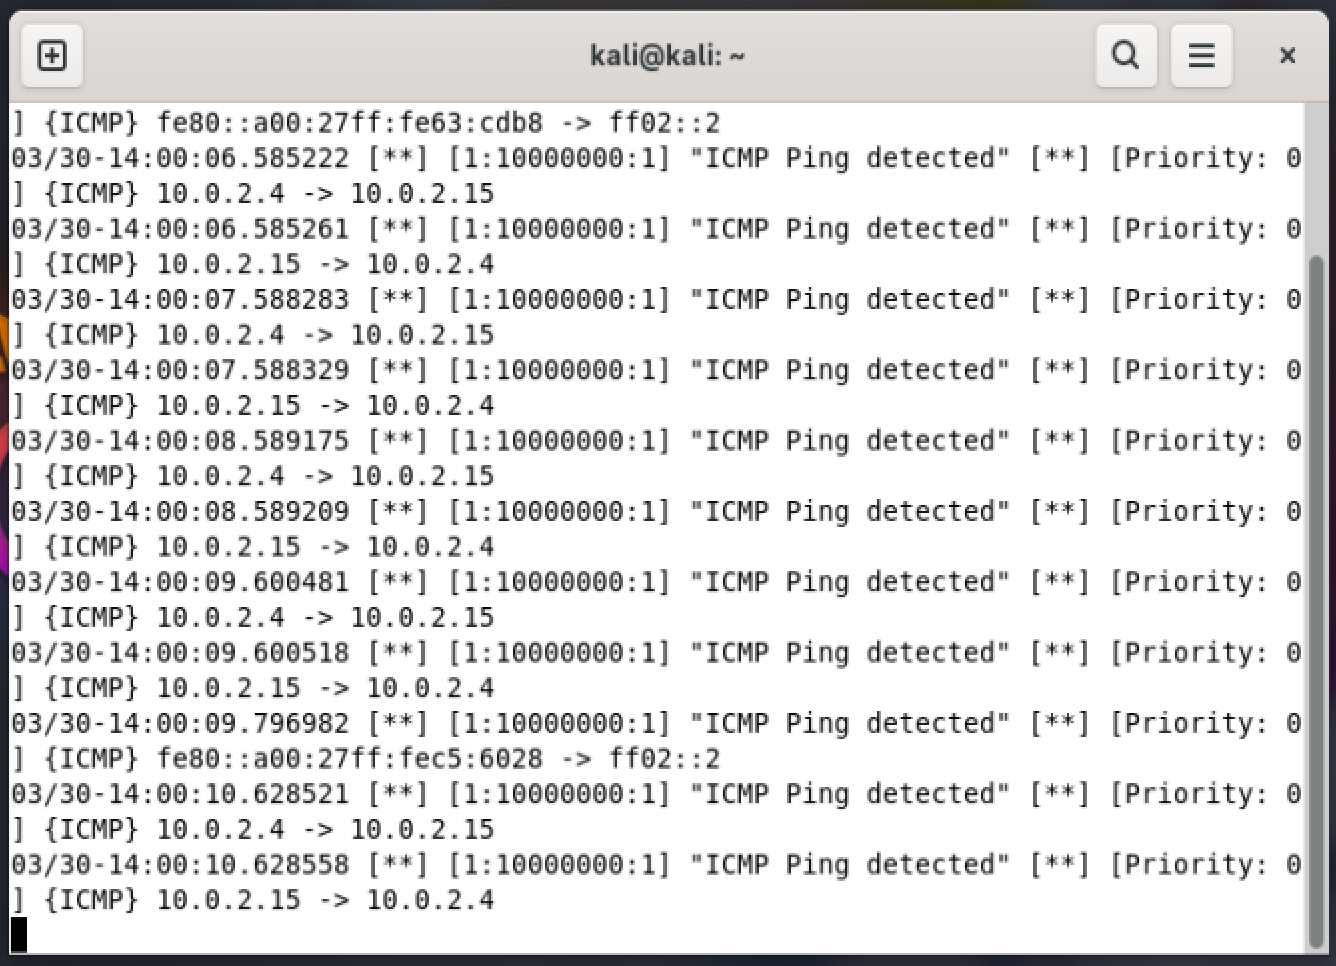
\includegraphics[width=\textwidth]{images/d1.1.png}\\
\textit{Figure 1. Screenshot of Snort detecting ICMP pings from Ubuntu VM.}

\newpage

\section{Writing Detection Rules}

\subsection{Port Scan Detection}
\begin{itemize}
	\item \textbf{alert tcp any any -$>$ \$HOME\underbar{   }NET any (msg:"PORT SCAN DETECTED - TCP SYN Flood"; flags:S; detection\underbar{   }filter:track by\underbar{   }src, count 20, seconds 5; sid:1000001; rev:1;)}
	\item 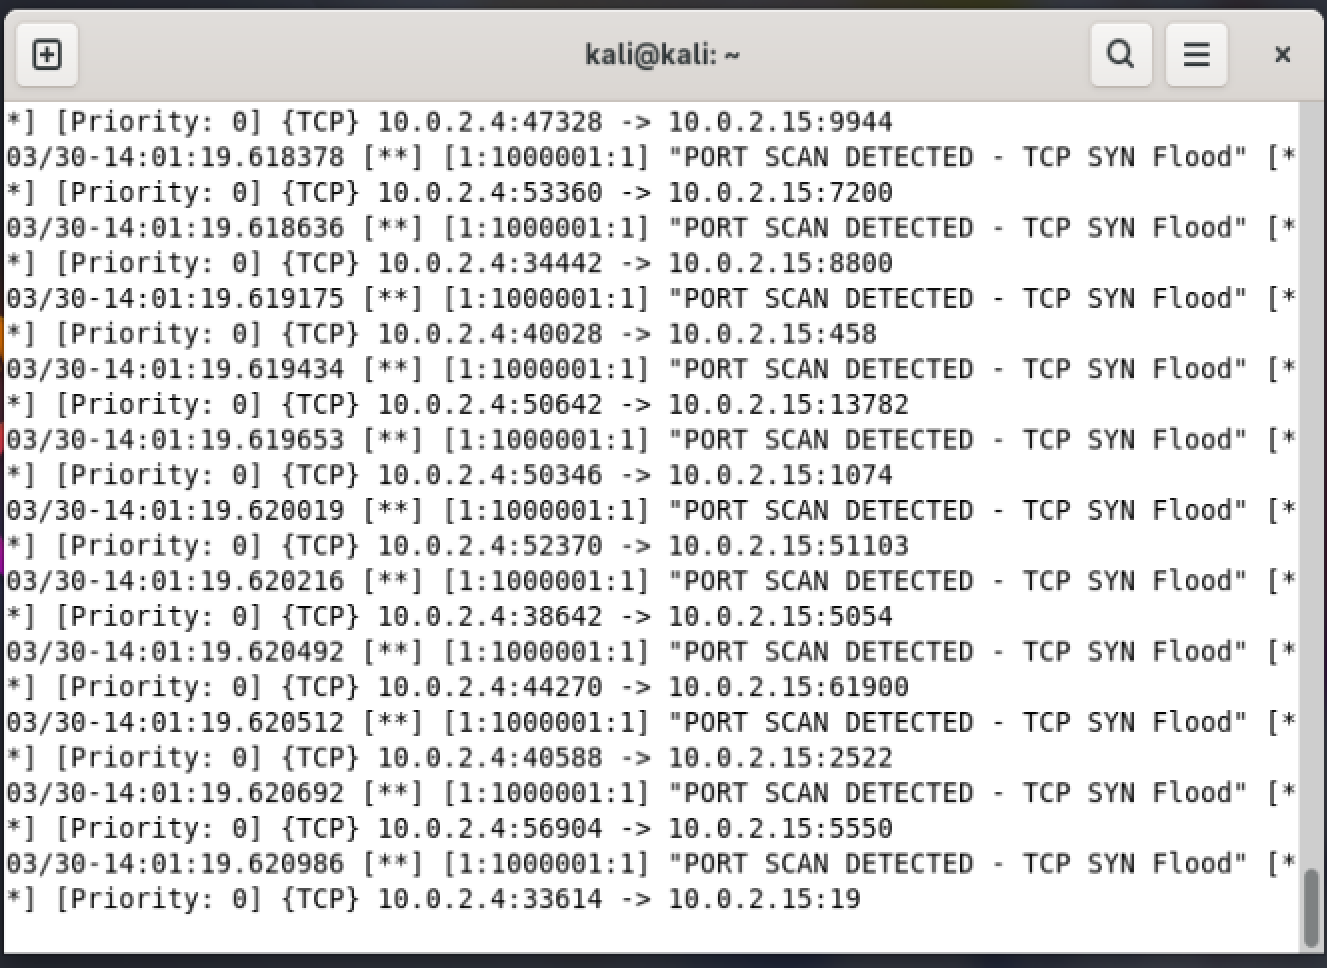
\includegraphics[width=0.95\textwidth]{images/d2.1.png}\\
		\textit{Figure 2. Snort alert for TCP SYN flood port scan.}
	\item Setting the threshold to 20 packets in 5 seconds attempts to strike a balance between potentially having regular traffic trigger a warning when set too low and letting a clever attacker use more deliberate scans that delay allow them to limit scan rates and stay under the radar. Since a default Nmap scan blasts through 100s of ports in seconds, this threshold should easily catch suspect activity while allowing normal activity to move quietly.
\end{itemize}

\subsection{SSH Brute Force Detection}
\begin{itemize}
	\item  \textbf{alert tcp any any -$>$ \$HOME\underbar{   }NET 22 (msg:"SSH BRUTE FORCE DETECTED - Multiple Connection Attempts"; flags:S; detection\underbar{   }filter:track by\underbar{   }src, count 5, seconds 10; sid:1000002; rev:1;)}
	\item 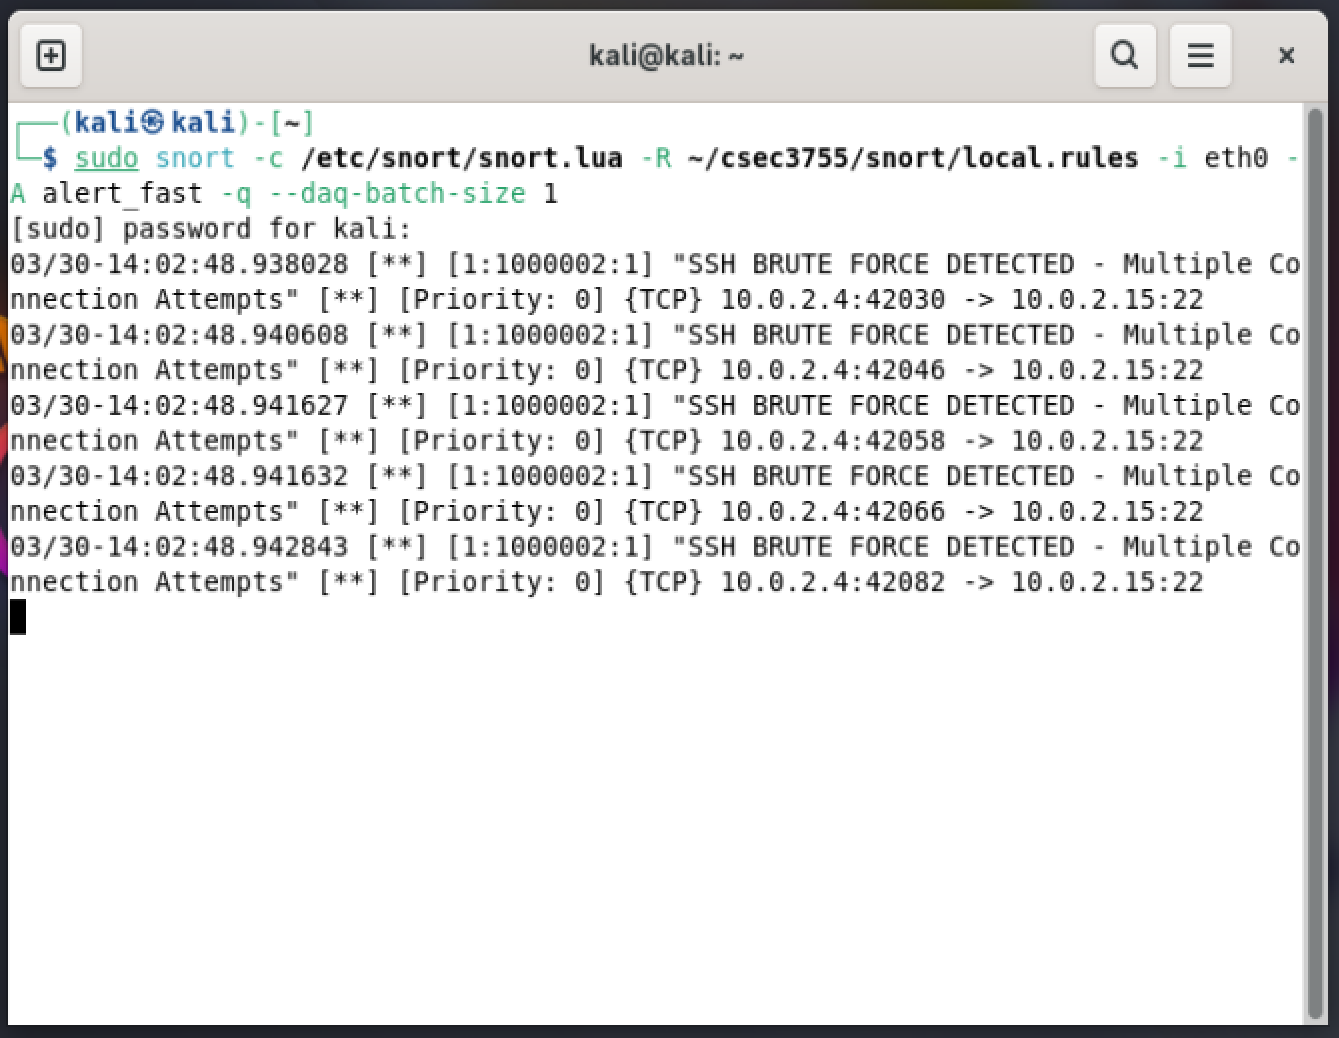
\includegraphics[width=0.95\textwidth]{images/d2.2.png}\\
		\textit{Figure 3. Snort alert for SSH brute force attack.}
	\item I got to experience this first hand as my initial commands to the Kali machine would just keep me in a login loop. With or without the password, the time it took for the machine to check the password entered made it so the attempts were not picked up. It was only after I had Claude write up a quick command to simulate the attack that we saw the alert go off. This was a good first-hand show that an attacker would have to slow down to a snail's pace to go undetected.
\end{itemize}

\subsection{Custom Content Rule}
\begin{itemize}
	\item \textbf{alert tcp any any -$>$ \$HOME\underbar{   }NET 80 (msg:"SQL INJECTION DETECTED - SQL Keyword Found"; flow:to\underbar{   }server,established; pcre:"/SELECT|UNION|DROP/i"; sid:1000003; rev:1;)}
	\item 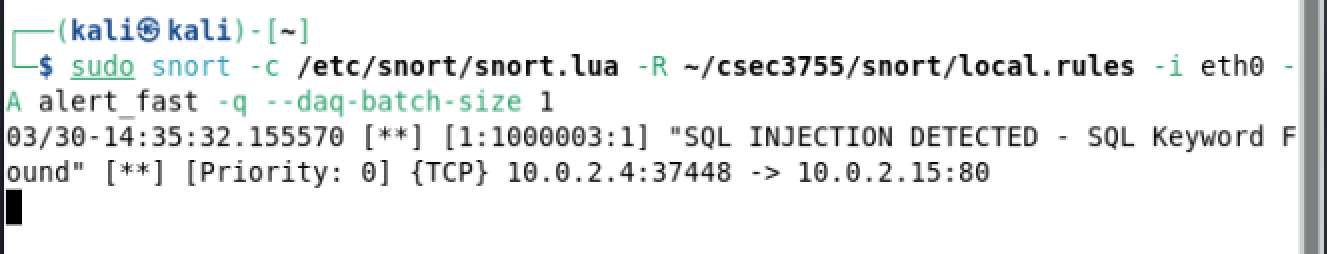
\includegraphics[width=0.95\textwidth]{images/d2.3.png}\\
		\textit{Figure 4. Snort alert for SQL injection attempt of keywords SELECT, UNION, and DROP.}
	\item This rule detects the use of common SQL keywords SELECT, UNION, and DROP. These keywords are often used in SQL injection attacks to retrieve data (SELECT), combine results (UNION), or delete data (DROP). This rule should not generate false positives for normal web traffic since these keywords are unlikely to appear in typical HTTP requests.
\end{itemize}

\newpage

\section{Alert Analysis}
\textbf{Alert Output:}\\
\$ sudo snort -c /etc/snort/snort.lua -R ~/csec3755/snort/local.rules -i eth0 -A alert\underbar{   }fast -q --daq-batch-size 1 \\                  
sudo password for kali: \\
03/30-17:30:32.360484 [**] [1:1000002:1] "SSH BRUTE FORCE DETECTED - Multiple Connection Attempts" [**] [Priority: 0] {TCP} 10.0.2.4:34480 -$>$ 10.0.2.15:22\\
03/30-17:30:32.366998 [**] [1:1000002:1] "SSH BRUTE FORCE DETECTED - Multiple Connection Attempts" [**] [Priority: 0] {TCP} 10.0.2.4:34490 -$>$ 10.0.2.15:22\\
03/30-17:30:32.368117 [**] [1:1000002:1] "SSH BRUTE FORCE DETECTED - Multiple Connection Attempts" [**] [Priority: 0] {TCP} 10.0.2.4:34506 -$>$ 10.0.2.15:22\\
03/30-17:30:32.369264 [**] [1:1000002:1] "SSH BRUTE FORCE DETECTED - Multiple Connection Attempts" [**] [Priority: 0] {TCP} 10.0.2.4:34516 -$>$ 10.0.2.15:22\\
03/30-17:30:32.370099 [**] [1:1000002:1] "SSH BRUTE FORCE DETECTED - Multiple Connection Attempts" [**] [Priority: 0] {TCP} 10.0.2.4:34530 -$>$ 10.0.2.15:22\\
03/30-17:30:42.169653 [**] [1:1000003:1] "SQL INJECTION DETECTED - SQL Keyword Found" [**] [Priority: 0] {TCP} 10.0.2.4:34166 -$>$ 10.0.2.15:80\\
03/30-17:30:47.205335 [**] [1:10000000:1] "ICMP Ping detected" [**] [Priority: 0] {ICMP} fe80::a00:27ff:fe63:cdb8 -$>$ ff02::2\\
03/30-17:32:43.769580 [**] [1:10000000:1] "ICMP Ping detected" [**] [Priority: 0] {ICMP} fe80::a00:27ff:fe63:cdb8 -$>$ ff02::2\\
03/30-17:36:31.609834 [**] [1:10000000:1] "ICMP Ping detected" [**] [Priority: 0] {ICMP} fe80::a00:27ff:fe63:cdb8 -$>$ ff02::2\\


\subsection{Alert 1: SSH Brute Force Attack}
\textbf{Alert Output:}\\
03/30-17:30:32.370099 [**] [1:1000002:1] "SSH BRUTE FORCE DETECTED - Multiple Connection Attempts" [**] [Priority: 0] {TCP} 10.0.2.4:34530 -$>$ 10.0.2.15:22
\\
\ \\
\textbf{Analysis:}
{\singlespacing
	\begin{longtable}{
 		||>{\raggedright\arraybackslash}p{\colSmall}
  		| >{\raggedright\arraybackslash}p{\colBig}||}
		\hline
  	    	 \textbf{SID and Revision} & [1:1000002:1] \\
			 \hline
			 \textbf{Alert Message} & "SSH BRUTE FORCE DETECTED - Multiple Connection Attempts" \\
			 \hline
			 \textbf{Source IP and Port} & 10.0.2.4:34530 \\
			 \hline
			 \textbf{Destination IP and Port} & 10.0.2.15:22 \\
			 \hline
			 \textbf{Timestamp} & 03/30-17:30:32.370099 \\
			 \hline
			 \textbf{Priority/ Classification} & 0 \\
		\hline
	\end{longtable}
}

\subsection {Alert 2: SQL Injection Attempt}
\textbf{Alert Output:}\\
03/30-17:30:42.169653 [**] [1:1000003:1] "SQL INJECTION DETECTED - SQL Keyword Found" [**] [Priority: 0] {TCP} 10.0.2.4:34166 -> 10.0.2.15:80\\
\ \\
\textbf{Analysis:}
{\singlespacing
	\begin{longtable}{
 		||>{\raggedright\arraybackslash}p{\colSmall}
  		| >{\raggedright\arraybackslash}p{\colBig}||}
		\hline
  	    	 \textbf{SID and Revision} & [1:1000003:1] \\
			 \hline
			 \textbf{Alert Message} & "SQL INJECTION DETECTED - SQL Keyword Found" \\
			 \hline
			 \textbf{Source IP and Port} & 10.0.2.4:34166 \\
			 \hline
			 \textbf{Destination IP and Port} & 10.0.2.15:80 \\
			 \hline
			 \textbf{Timestamp} & 03/30-17:30:42.169653 \\
			 \hline
			 \textbf{Priority/ Classification} & 0 \\
		\hline
	\end{longtable}
}
\newpage
\subsection{Overview:}
\par When taking an overview of the Snort outputs, my immediate attention turns to the SSH brute force warnings. The five rapid connection attempts are textbook signs of a potential credential stuffing attack and represents a clear, active threat. If successful, the attacker would have full control of the machine. The SQL injection alerts would be my second priority, although they do present an ugent threat as even a few show that an attacker could be probing for vulnerabilities, a success meaning leaked or damaged data. Finally, I would look at the ICMP alerts, although those are just signs of normal discovery traffic. They are more of an indicator that the rule should be tightened up a little and are a good example of false positives.  

\section{Reflection Questions}

\subsection{IDS \& Firewall:}


\subsection{False Positives:}
\par The rule as it stands just alerts us to every ping that is detected, so we just have to turn it down a little. We can add itype:8 to match ICMP Echo Requests only and ignore router discovery and multicast traffic. Additionally, we can add detection\underbar{   }filter:track by\underbar{   }src, count 5, seconds 3 to the rule to only pay attention to multiple pings in quick succession from the same source.

\subsection{The Target Lesson:}

\vfill
\textit{++report written with (minimal) help from Claude (Sonnet 4.6)}
\end{document}

% +++++++++ Helpful stuff +++++++++++
%
% +++ Using Minipages +++
% \begin{minipage}[t]{\linewidth}
% \includegraphics[width=0.50\textwidth]{*Image file}\\
% \textit{*Image subtitle}
% \end{minipage}
% \end{enumerate}
%


% +++ Fixed width table +++
%\begin{tabularx}{1.0\textwidth}{
%	|| >{\raggedright\arraybackslash}X
%	|  >{\raggedright\arraybackslash}X
%	|  >{\raggedright\arraybackslash}X
%	|  >{\raggedright\arraybackslash}X || }
%	\hline
%	\textbf{x} & \textbf{x} & \textbf{x} & \textbf{x} \\
%	\hline \hline
%	x $ x $ x & x & x & x  \\
%	\hline
%	x $ x $ x & x & x & x \\
%	\hline
%	x $ x $ x & x & x & x \\
%	\hline
%	x $ x $ x & x &  x  & x \\
%	\hline
%\end{tabularx}
%

% +++ For tables that take multiple pages +++
%{\singlespacing
%	\begin{longtable}{
% 		|| >{\centering\arraybackslash}p{\colNum}
%  		| >{\raggedright\arraybackslash}p{\colSmall}
%  		| >{\raggedright\arraybackslash}p{\colSmall}
%  		| >{\raggedright\arraybackslash}p{\colBig}
%  		| >{\raggedright\arraybackslash}p{\colSmall} ||}
%		\hline
%		\textbf{x} & \textbf{x} & \textbf{x} & \textbf{x} & \textbf{x} \\
%		\hline\hline
%		\endhead
%		\hline
%  	    	 x & x & x & x  & x \\
%		\hline
%	\end{longtable}
%}












